\documentclass[Main]{subfiles}
\begin{document}



\chapter{Eksterne grænseflader}

\section{Brugergrænseflade}
Brugerens kontakt med dronen består i strømtilslutning mellem batteriet og dronen selv.
Foruden dette har brugeren også en fjernbetjening, illustreret på Figur 

\begin{figure}[H]
\centering
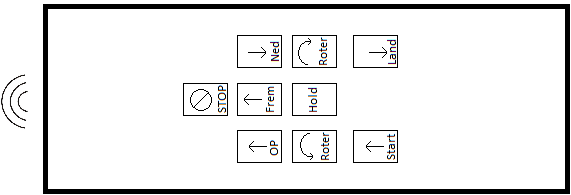
\includegraphics[scale=0.8, angle=270]{Print}
\caption{Illustration af fjernbetjeningen}
\label{Fig:Fjernbetjening}
\end{figure}





\section{Software-grænseflade}
Systemet bygger på et ikke-modificeret open source bibliotek, Arduino\cite{Arduino}, samt en modificeret FIFO-klasse\cite{FIFO}, QueueList\cite{QueueList}.


Dronens software bygger desuden oven på Aeroquads open source projekt\cite{AQ-software}, der er kraftigt modificeret for den nødvendige udbygning.






%\chapter{Krav til ydelse}
%Følgende er krav til dronen og styringen af denne:
%
%	\begin{itemize}
%	\item Drone kan flyve i minimum 10 minutter.
%	\item Drone skal kunne flyve med en hastighed på 25 $\dfrac{cm}{s}$.
%	\end{itemize}






\chapter{Kvalitetsfaktorer}
Kvalitetsfaktorer til systemet hviler primært på pålideligheden af signalet mellem fjernbetjeningen og dronen, samt muligheden for videreudvikling for andre.
\\
Kommunikationen fra fjernbetjeningen bygges derfor således, at den kan variere i størrelse, men også at alle pakker bliver sendt til og modtaget af dronen.
Fjernbetjeningen kan derfor sende forskellige typer af signaler til dronen afhængigt af, hvad brugeren ønsker dronen skal reagere på.
\\
Modtagerdelen på dronen er designet således, at det ser på typen af det indkommende signal og reagerer derpå.
Dette giver mulighed for mange ikke blot at modtage forskellige programmer, der skal eksekveres enkeltvis, men også programsekvenser, poke-signaler for signalstyrke mm.











\chapter{Myndighedskrav}
Regler for flyvning med drone gælder følgende:

\begin{itemize}
\item Flyvningen må ikke udsætte andres liv og ejendom for fare\cite[s. 1]{Lov1}.
\item Flyvning skal foregå mindst 5 km fra banerne på en offentlig flyveplads og mindst 8 km fra banerne på en militærflyvestation\cite[s. 1]{Lov1}.
\item Afstanden til bymæssig bebyggelse og større offentlig vej skal være mindst 150 m\cite[s. 1]{Lov1}.
\item Flyvehøjden må højst være 100 m over terræn\cite[s. 2]{Lov1}.
\item Tæt bebyggede områder, (bl.a. sommerhusområder og beboede campingpladser), samt områder, hvor et større antal mennesker er samlet i fri luft, må ikke overflyves\cite[s. 2]{Lov1}.
\item Særligt følsomme naturområder må ikke overflyves\cite[s. 2]{Lov1}.
\end{itemize} 


\end{document}